\chapter{實驗結果討論與錯誤分析}
使用額外資料訓練的結果會在附錄中以表格呈現。

\section{實驗一:比較 Ratio Mask 與 Wiener Filter 的效果比較}
U-Net6(baseline)為學長提出的架構,且使用所有第三章提及過的資料集訓練。以 U-Net6(base)為基準,在後處理的時候做 mulitchannel Wiener filter 與 ratio mask filter,以 museval 檢測(見表\ref{filter_result_table} 與圖\ref{filter_result1} )。在聆聽觀察中,濾波前的伴奏預測軌會有毛邊感(fuzzy sound),為無法完美去除的主唱音軌導致。由圖\ref{filter_result2} 上的主唱軌聲波可明顯看出,濾波可以明顯的提升輸出的效果。mulitchannel Wiener filter 與 ratio mask filter 並無太大差異,但因為實現的細節不同,前者在伴奏軌的效果會比較好,但在聽感上並無太大差異。

\begin{table}[htbp]
\centering
\resizebox{\textwidth}{!}{%
\begin{tabular}{|r|ccc|ccc|}
\hline
 &  & 主唱軌 &  &  & 伴奏軌 &  \\ \hline
 & \multicolumn{1}{c|}{\textbf{SDR}} & \multicolumn{1}{c|}{SIR} & SAR & \multicolumn{1}{c|}{\textbf{SDR}} & \multicolumn{1}{c|}{SIR} & \textbf{SAR} \\ \hline
U-Net6  (baseline) & \multicolumn{1}{c|}{7.269} & \multicolumn{1}{c|}{15.045} & 7.224 & \multicolumn{1}{c|}{13.805} & \multicolumn{1}{c|}{16.785} & 14.520 \\ \hline
U-Net6  (baseline) w/ MWF & \multicolumn{1}{c|}{\textbf{7.648}} & \multicolumn{1}{c|}{18.593} & 7.436 & \multicolumn{1}{c|}{\textbf{14.288}} & \multicolumn{1}{c|}{20.332} & \textbf{14.815} \\ \hline
U-Net6  (baseline) w/ ratio mask filter & \multicolumn{1}{c|}{\textbf{7.648}} & \multicolumn{1}{c|}{18.585} & 7.435 & \multicolumn{1}{c|}{14.194} & \multicolumn{1}{c|}{20.221} & 14.758 \\ \hline
\end{tabular}%
}
\caption{實驗數據表}
\label{filter_result_table}
\end{table}

\begin{figure}[htbp]
    \hfil
    \begin{minipage}[t]{1.0\textwidth}
        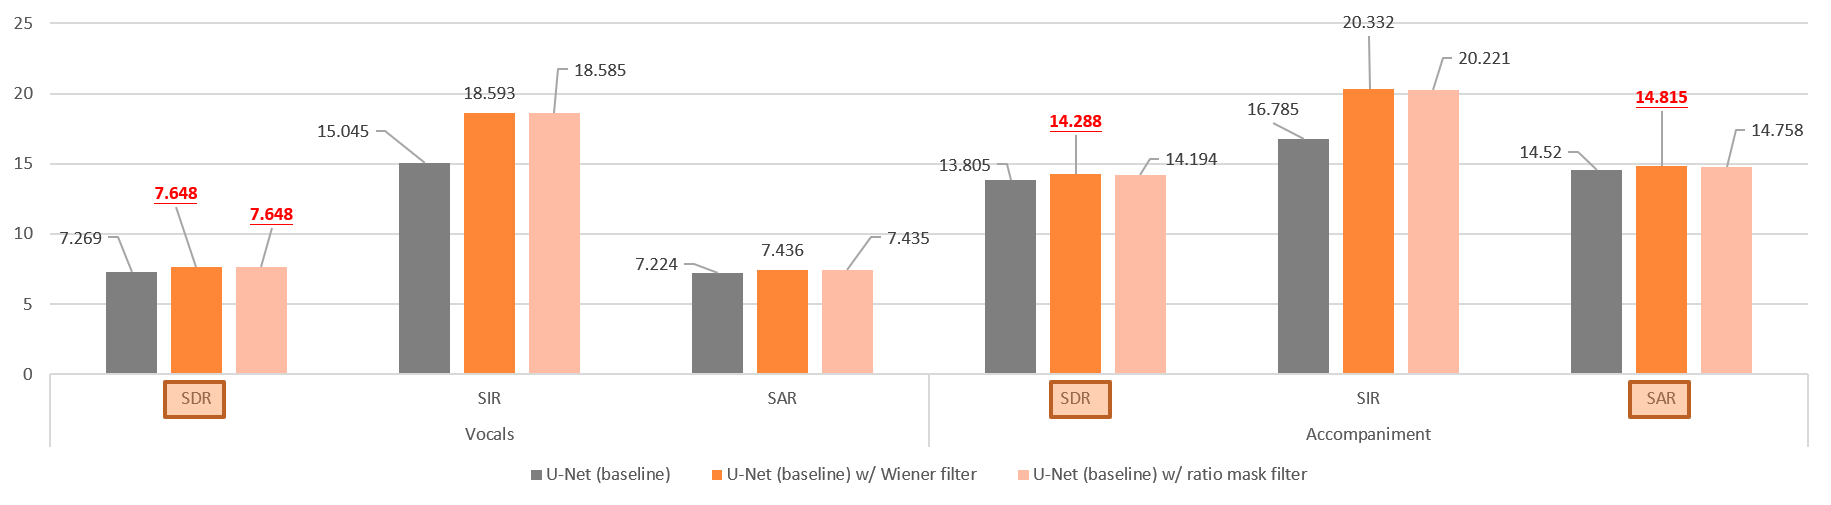
\includegraphics[width=\textwidth]{./figures/chapter05_result/filter_result1.png}
        \caption {濾波實驗長條圖}
        \label{filter_result1}
    \end{minipage}
    \hfil
\end{figure}

\begin{figure}[htbp]
    \hfil
    \begin{minipage}[t]{1.0\textwidth}
        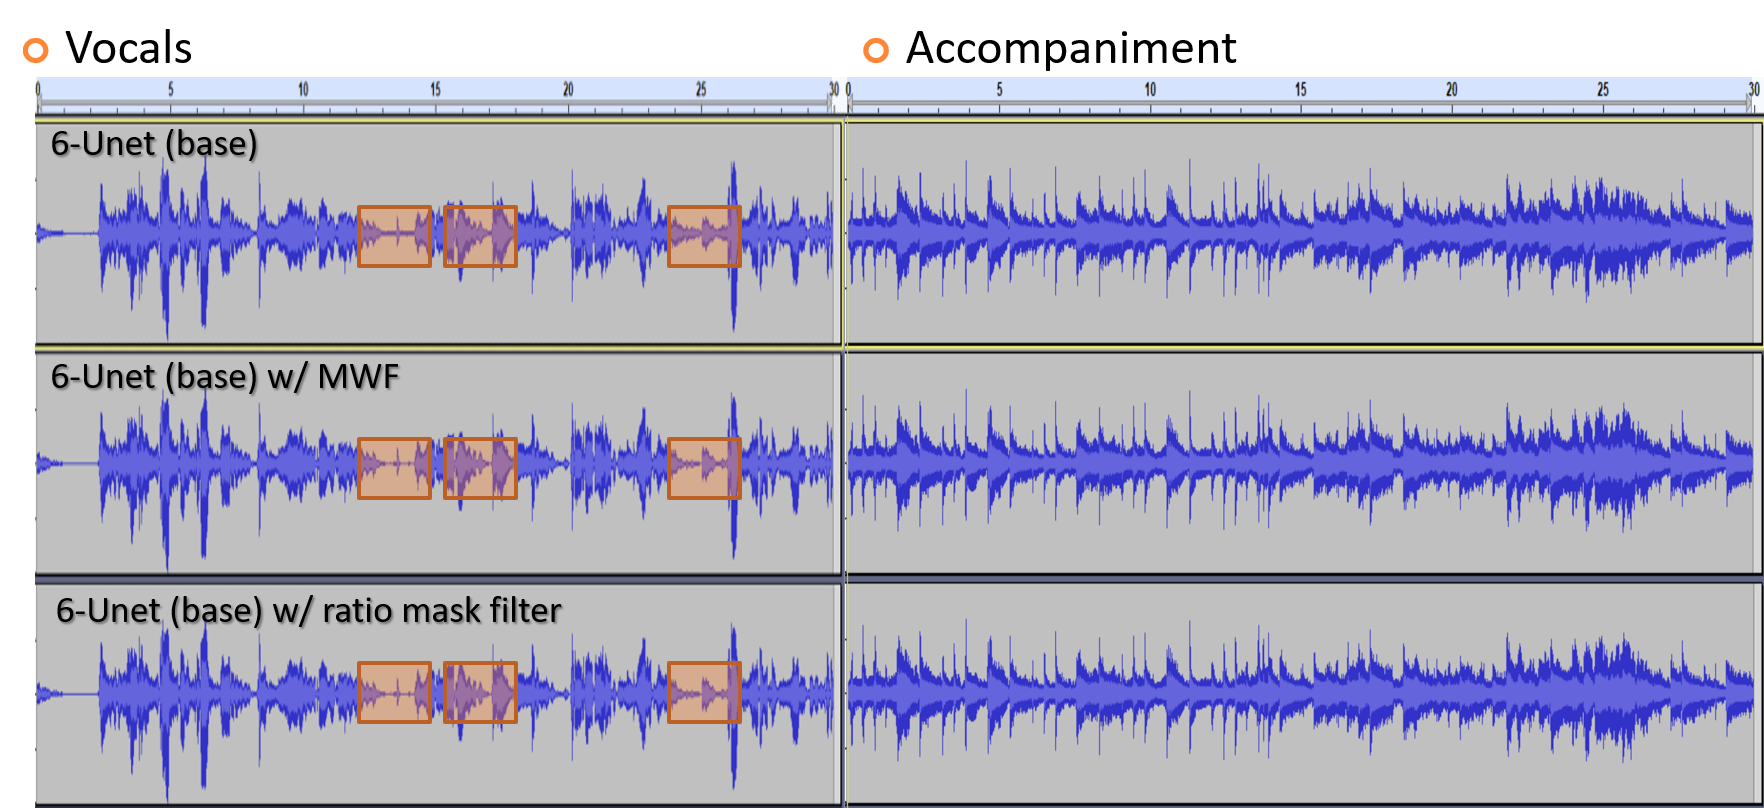
\includegraphics[width=\textwidth]{./figures/chapter05_result/filter_result2.png}
        \caption {濾波實驗效果圖}
        \label{filter_result2}
    \end{minipage}
    \hfil
\end{figure}

\clearpage

\section{實驗二:頻譜刪減法效果比較}
% 補 nn 方法的 alpha_f 圖
此實驗是基於先前實驗的效果,在 $\alpha=0.2$ 的時候,其效果有些許地增幅,但這是對於每個 frequency bin 都使用同一個頻譜刪減幅度,本輪文提出兩個方法希望可對每個 $f \in F$ 各自求取最好的刪減幅度 $\alpha$,其效果以 museval 做檢測(見表\ref{magnitude_subtraction_method_table} 與圖\ref{magnitude_subtraction_method_result1})。

\begin{table}[htbp]
\centering
\resizebox{\textwidth}{!}{%
\begin{tabular}{|r|ccc|ccc|c|}
\hline
 &  & 主唱軌 &  &  & 伴奏軌 &  & Note \\ \hline
 & \multicolumn{1}{c|}{\textbf{SDR}} & \multicolumn{1}{c|}{SIR} & SAR & \multicolumn{1}{c|}{\textbf{SDR}} & \multicolumn{1}{c|}{SIR} & \textbf{SAR} &  \\ \hline
\textit{U-Net6 (baseline)} & \multicolumn{1}{c|}{\textit{7.269}} & \multicolumn{1}{c|}{\textit{15.045}} & \textit{7.224} & \multicolumn{1}{c|}{\textit{13.085}} & \multicolumn{1}{c|}{\textit{16.785}} & \textit{14.751} &  \\ \hline
0.2 as ratio for each bins & \multicolumn{1}{c|}{\textbf{7.352}} & \multicolumn{1}{c|}{18.748} & 7.146 & \multicolumn{1}{c|}{\textbf{14.031}} & \multicolumn{1}{c|}{20.728} & 14.151 & 先前實驗 \\ \hline
Band-based optimal ratio & \multicolumn{1}{c|}{7.346} & \multicolumn{1}{c|}{16.077} & 7.507 & \multicolumn{1}{c|}{13.988} & \multicolumn{1}{c|}{19.185} & 14.147 & 本次實驗 \\ \hline
Frequency-based optimal ratio & \multicolumn{1}{c|}{7.340} & \multicolumn{1}{c|}{15.704} & 7.345 & \multicolumn{1}{c|}{13.895} & \multicolumn{1}{c|}{17.151} & \textbf{14.634} & 本次實驗 \\ \hline
\end{tabular}%
}
\caption{頻譜刪減幅度實驗比較表}
\label{magnitude_subtraction_method_table}
\end{table}

\begin{figure}[htbp]
    \hfil
    \begin{minipage}[t]{1.0\textwidth}
        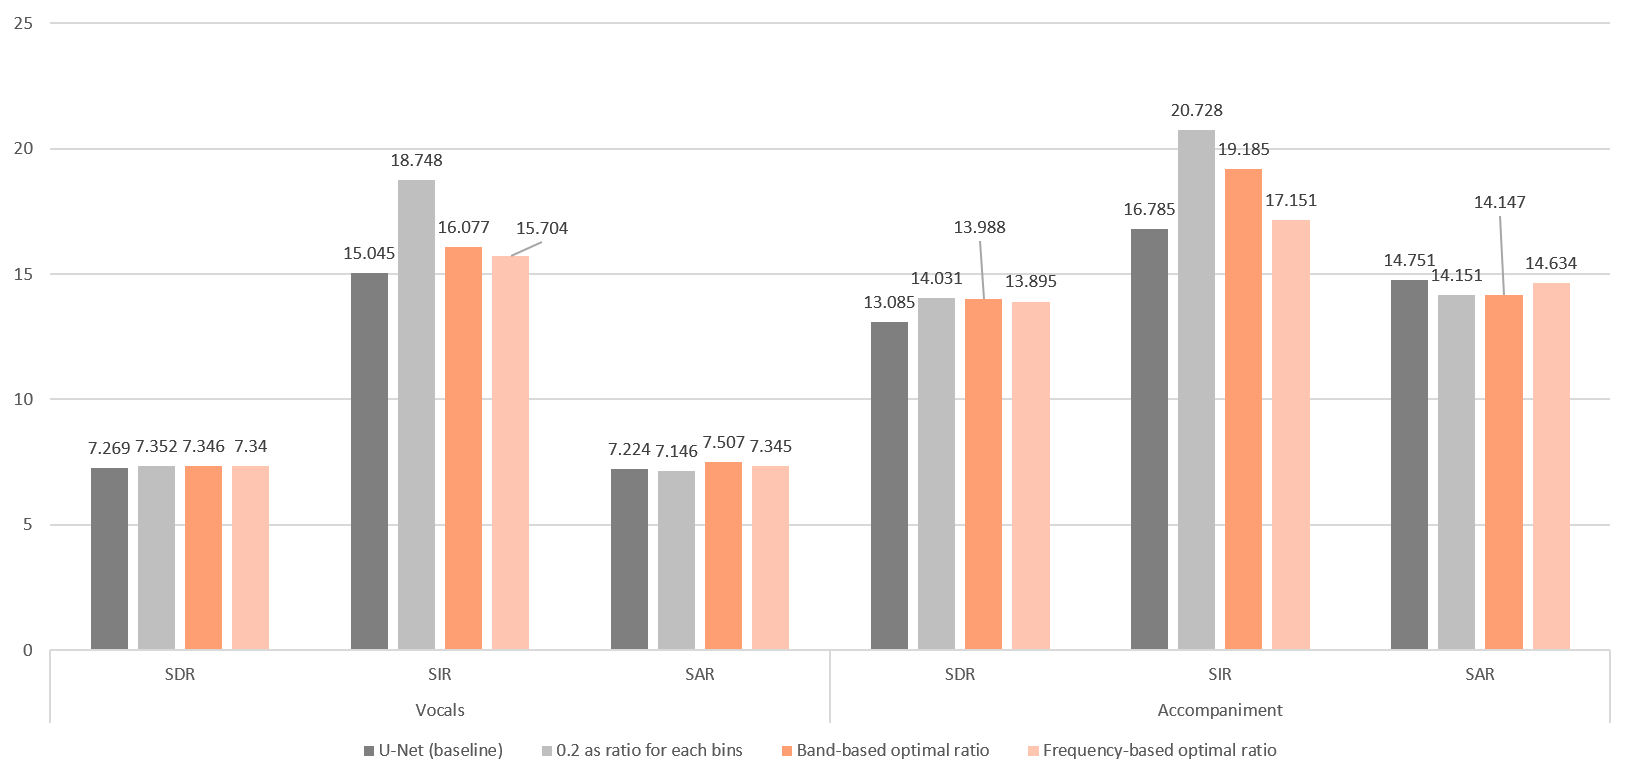
\includegraphics[width=\textwidth]{./figures/chapter05_result/magnitude_subtraction_method_result1.png}
        \caption {頻譜刪減幅度實驗比較表}
        \label{magnitude_subtraction_method_result1}
    \end{minipage}
    \hfil
\end{figure}

第一個方法對於每個頻帶 $b\in Bands$ 求取頻譜刪減幅度 $\alpha_b$,圖\ref{magnitude_subtraction_method_result2} 表示出對應的刪減幅度值,左為主唱軌的刪減幅度,右為伴奏軌的刪減幅度。

\begin{figure}[htbp]
    \hfil
    \begin{minipage}[t]{0.6\textwidth}
        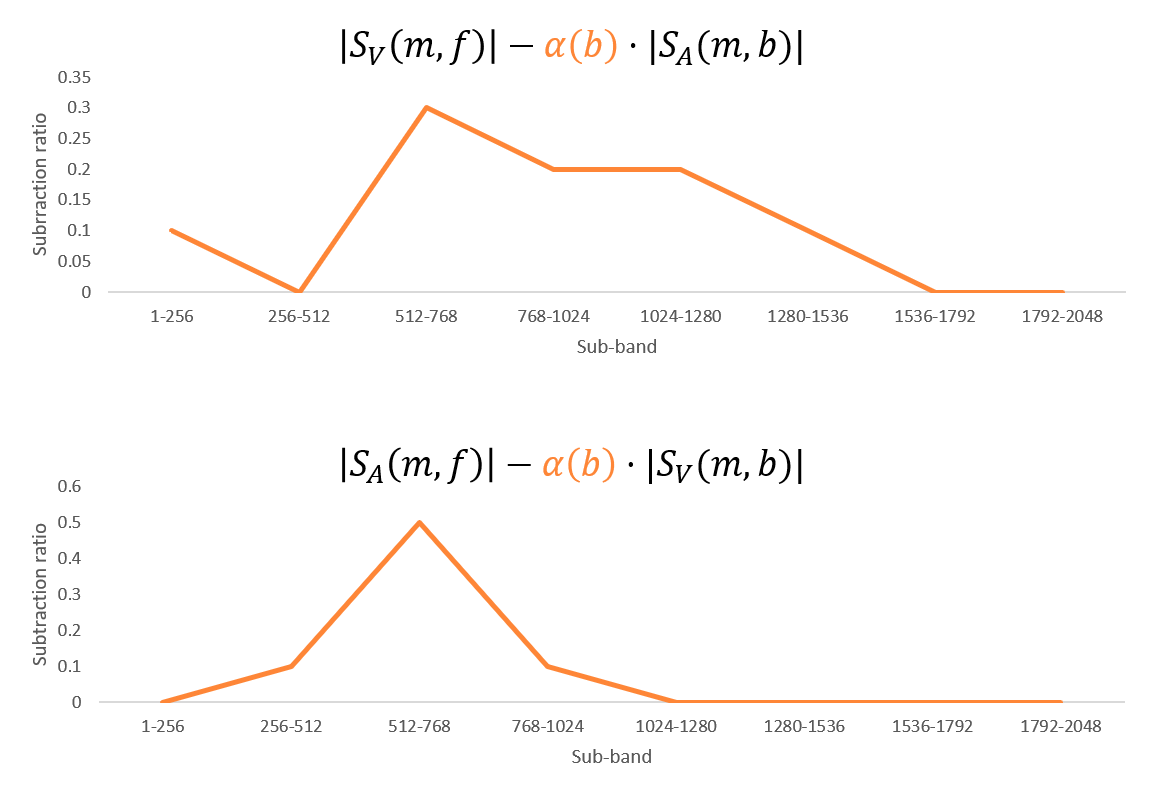
\includegraphics[width=\textwidth]{./figures/chapter05_result/magnitude_subtraction_method_result2.png}
        \caption {實驗方法一取得的各個 $\alpha_b$}
        \label{magnitude_subtraction_method_result2}
    \end{minipage}
    \hfil
\end{figure}

第二個方法對於每個 $f\in F$ 求取頻譜刪減幅度 $\alpha_f$,圖\ref{magnitude_subtraction_method2_result1} 與圖\ref{magnitude_subtraction_method2_result2}  表示出對應的刪減幅度值,圖\ref{magnitude_subtraction_method2_result1} 為主唱軌被刪減時乘上的幅度,圖\ref{magnitude_subtraction_method2_result2} 為伴奏軌被刪減時乘上的幅度。

\begin{figure}[htbp]
    \hfil
    \begin{minipage}[t]{0.6\textwidth}
        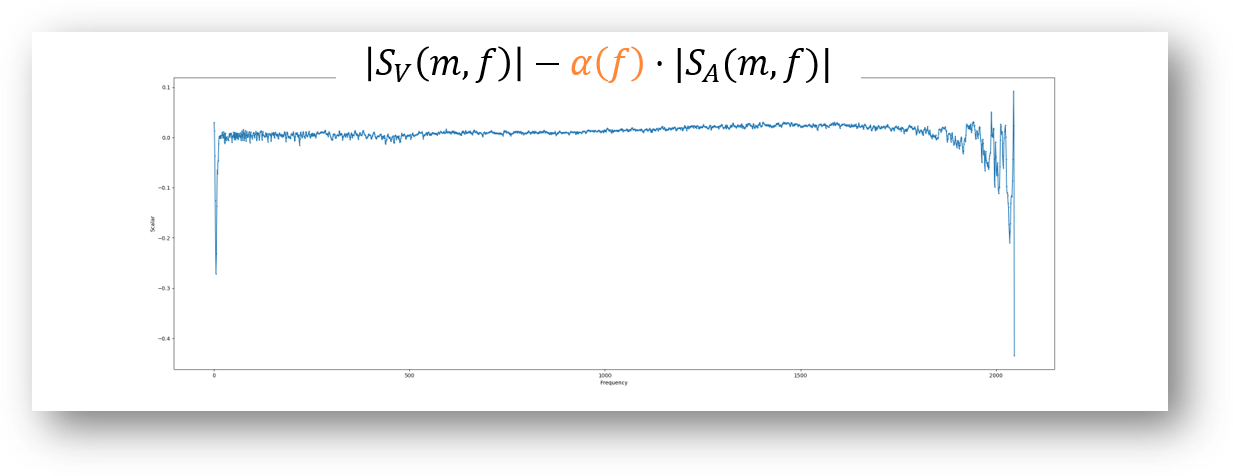
\includegraphics[width=\textwidth]{./figures/chapter05_result/spectrogram_subtraction_nn_accompaniment-vocals_T-216.png}
        \caption {實驗方法二取得的各個 $\alpha_f$}
        \label{magnitude_subtraction_method2_result1}
    \end{minipage}
    \hfil
\end{figure}
\begin{figure}[htbp]
    \hfil
    \begin{minipage}[t]{0.6\textwidth}
        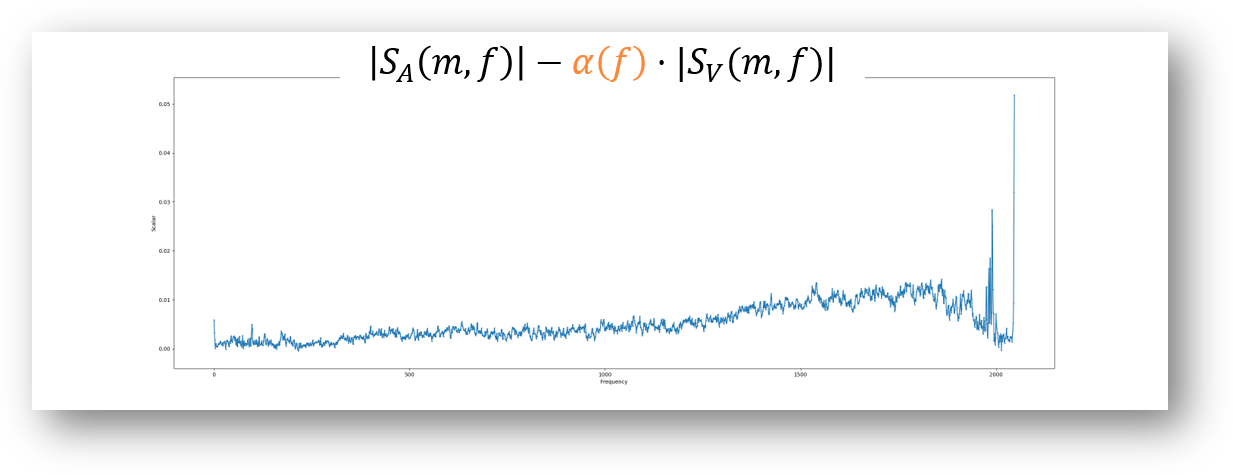
\includegraphics[width=\textwidth]{./figures/chapter05_result/spectrogram_subtraction_nn_vocals-accompaniment_T-216.png}
        \caption {實驗方法二取得的各個 $\alpha_f$}
        \label{magnitude_subtraction_method2_result2}
    \end{minipage}
    \hfil
\end{figure}

在 frequency-based optimal ratio 實驗中, initial weight 對於梯度下降法也會有所影響,上面的結果是對 initial weight 設定為 0。在這邊作者另外嘗試對 initial weight 設定為 0.2 時的效果,可以觀察到,取得的 $\alpha_f$ (圖\ref{magnitude_subtraction_method2_result3}、圖\ref{magnitude_subtraction_method2_result4} )會有變化,但在效果來說,並沒有差異太大 (表\ref{frequency-based_init_weight_table}、圖\ref{magnitude_subtraction_method_result3})。

\begin{figure}[htbp]
    \hfil
    \begin{minipage}[t]{0.6\textwidth}
        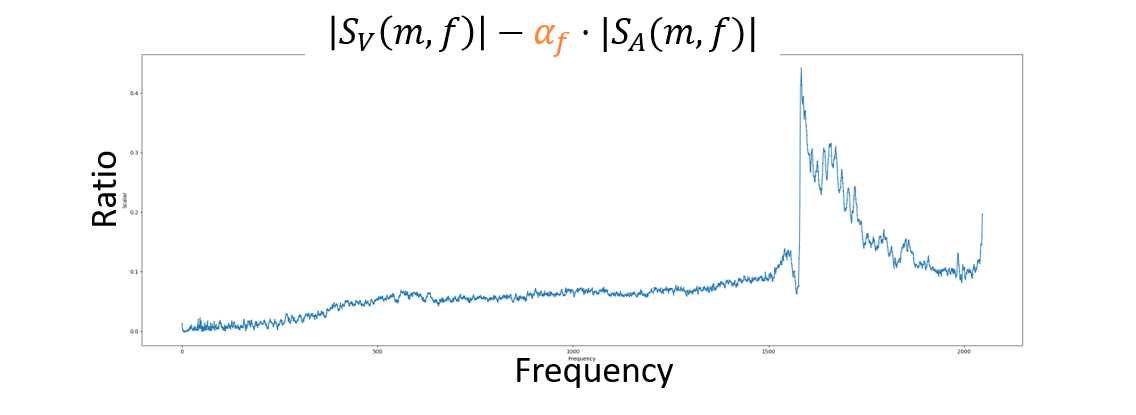
\includegraphics[width=\textwidth]{./figures/chapter05_result/init0.2_spectrogram_subtraction_nn_accompaniment-vocals_T-216.png}
        \caption {Initial weight 設為 0.2 時,frequency-based optimal ratio 取得到的 $\alpha_f$}
        \label{magnitude_subtraction_method2_result3}
    \end{minipage}
    \hfil
\end{figure}
\begin{figure}[htbp]
    \hfil
    \begin{minipage}[t]{0.6\textwidth}
        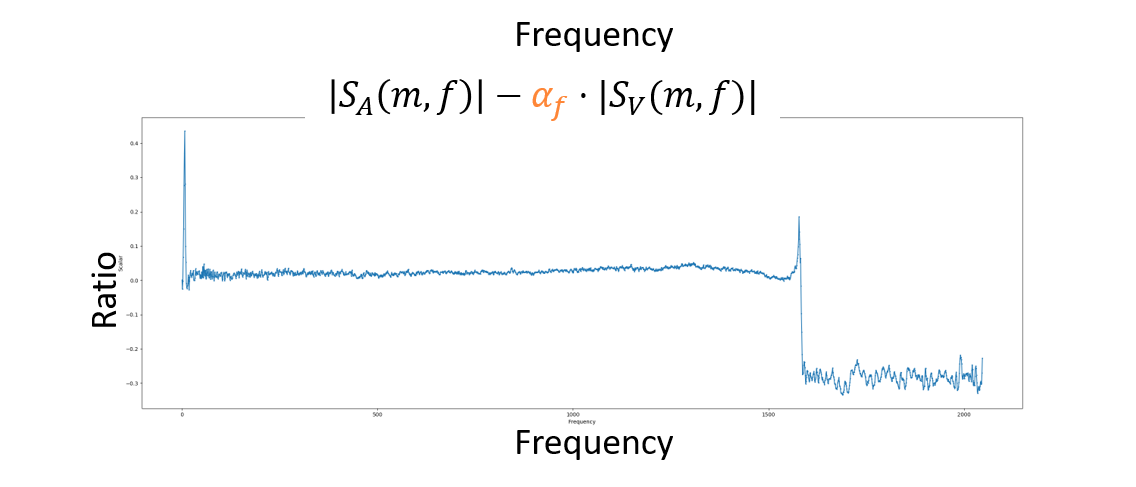
\includegraphics[width=\textwidth]{./figures/chapter05_result/init0.2_spectrogram_subtraction_nn_vocals-accompaniment_T-216.png}
        \caption {Initial weight 設為 0.2 時,frequency-based optimal ratio 取得到的 $\alpha_f$}
        \label{magnitude_subtraction_method2_result4}
    \end{minipage}
    \hfil
\end{figure}

\begin{table}[htbp]
\centering
\begin{tabular}{|r|c|c|c|c|c|c|}
\hline
\multicolumn{1}{|l|}{} & \multicolumn{3}{c|}{主唱軌} & \multicolumn{3}{c|}{伴奏軌} \\ \hline
\multicolumn{1}{|l|}{} & SDR & SIR & SAR & SDR & SIR & SAR \\ \hline
U-Net6 (baseline) & 7.269 & 15.045 & 7.224 & 13.085 & 16.785 & 14.751 \\ \hline
0.2 as ratio for each bins & 7.352 & 18.748 & 7.146 & 14.031 & 20.728 & 14.151 \\ \hline
w/ initial weight 0 & 7.34 & 15.704 & 7.345 & 13.895 & 17.151 & 14.634 \\ \hline
w/ initial weight 0.2 & 7.345 & 15.839 & 7.347 & 13.894 & 17.24 & 14.62 \\ \hline
\end{tabular}
\caption{Initial weight 設為 0.2 後的差異}
\label{frequency-based_init_weight_table}
\end{table}

\begin{figure}[htbp]
    \hfil
    \begin{minipage}[t]{1.0\textwidth}
        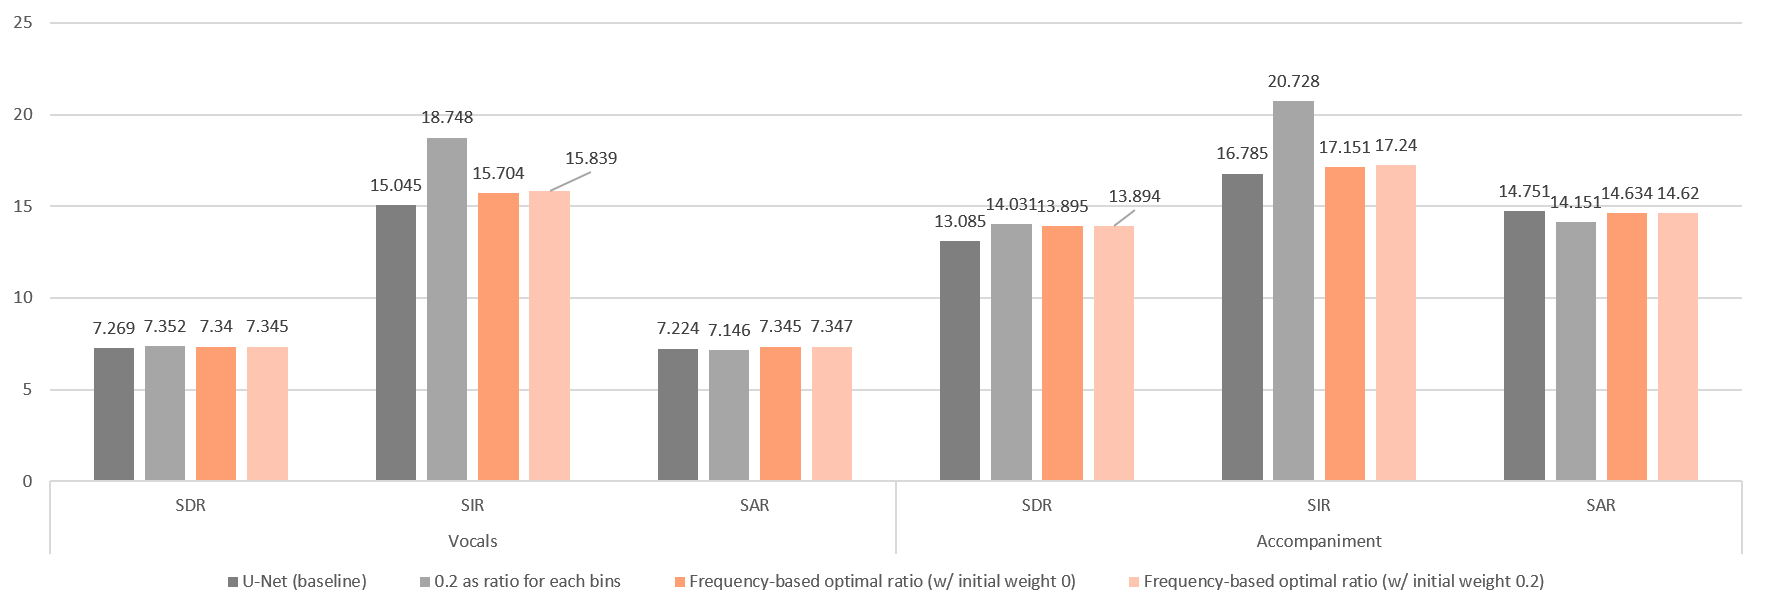
\includegraphics[width=\textwidth]{./figures/chapter05_result/magnitude_subtraction_method_result3.png}
        \caption {Initial weight 設為 0.2 後的差異}
        \label{magnitude_subtraction_method_result3}
    \end{minipage}
    \hfil
\end{figure}

\subsection*{錯誤分析}
與先前實驗的效果比較起來,本論文提出的方法雖有提升輸出音訊的效果,但無法勝過先前是必續探討的,本段落會提些見解,並在未來逐一克服。

關於第一個方法取得每個頻帶的刪減幅度 $\alpha_b$ ,其方法可能太過簡化,無法枚舉所有可能的排列組合,因為在找尋其中一個頻帶 $b_i$ 時,其餘的頻帶是不去考慮其刪減幅度,這可能也帶表了兩件事:區域的最佳解不能代表全域的解、區域枚舉的 $\alpha_{b_i}$ 粒度可能不夠細。可能使用 fmin search 的方式解此問題,直接定義其數學式找到最佳解,但這必須在未來慢慢探討。

關於第二個方法取得每個頻率的刪減幅度 $\alpha_f$,其問題也分成幾層面。第一個問題,可能架構根本就不適合此問題,需要再確認該輸入資訊的特性,以修改訓練的模型。第二個問題,是否只需第一種方式即可解決問題。這些必須在未來慢慢探討。

\clearpage

\section{實驗三:不同注意力模型效果比較}
修改原始模型中,U-Net6(baseline)程式維護度差與延展性差(No scalability )難以更改,因此先重新設計,轉換到另一個可維護且延展性好的 U-Net6\_s(convtranspose)。U-Net6 (AG) 與 U-Net6 (Sattn) 皆使用 U-Net6\_s(convtranspose)為基礎來開發(表\ref{attention_based_unet_table1}),架構在第四章以圖解釋。其中 U-Net6 (Sattn) 在伴奏預測效果最好(見表\ref{attention_based_unet_table2} 與圖\ref{attention_based_unet_result1}),但也是模型最龐大的,可以證明 self-attention 有助於時間軸上找到相同特徵序,聽感上,原本主唱預測軌難以去除的鼓聲也可以有效的解決(也可從圖\ref{U-Net6(baseline)_vocals} 與圖\ref{U-Net6(Sattn)_vocals} 上觀察頻譜中鼓在高頻能量已經消失,被 self-attention 的 U-Net 解決)。

\begin{figure}[htbp]
    \hfil
    \begin{minipage}[t]{0.45\textwidth}
        \centering
        % time series body
        \begin{tikzpicture}[scale=0.75]
        \begin{semilogyaxis} [
            xlabel = Epoch,
            ylabel = Loss,
        ]
            \addlegendentry{Training loss}
            \addplot table[mark=none, x=Step,y=Value, col sep=comma] {./numerical-data/chapter05_result/experiment03/6-Unet (base)/accompaniment/trnloss.csv};
            \addlegendentry{Validation loss}
            \addplot table[mark=none, x=Step,y=Value, col sep=comma] {./numerical-data/chapter05_result/experiment03/6-Unet (base)/accompaniment/valloss.csv};
        \end{semilogyaxis}
        \end{tikzpicture}
        % time series body
        \caption {U-Net (baseline) 對伴奏軌訓練的 loss}
        \label{e3:6-Unet (base):accompaniment}
    \end{minipage}
    \begin{minipage}[t]{0.45\textwidth}
        \centering
        % time series body
        \begin{tikzpicture}[scale=0.75]
        \begin{semilogyaxis} [
            xlabel = Epoch,
            ylabel = Loss,
        ]
            \addlegendentry{Training loss}
            \addplot table[mark=none, x=Step,y=Value, col sep=comma] {./numerical-data/chapter05_result/experiment03/6-Unet (base)/vocals/trnloss.csv};
            \addlegendentry{Validation loss}
            \addplot table[mark=none, x=Step,y=Value, col sep=comma] {./numerical-data/chapter05_result/experiment03/6-Unet (base)/vocals/valloss.csv};
        \end{semilogyaxis}
        \end{tikzpicture}
        % time series body
        \caption {U-Net6 (baseline) 對主唱軌訓練的 loss}
        \label{e3:6-Unet (base):vocals}
    \end{minipage}
    \hfil
\end{figure}


\begin{figure}[htbp]
    \hfil
    \begin{minipage}[t]{0.45\textwidth}
        \centering
        % time series body
        \begin{tikzpicture}[scale=0.75]
        \begin{semilogyaxis} [
            xlabel = Epoch,
            ylabel = Loss,
        ]
            \addlegendentry{Training loss}
            \addplot table[mark=none, x=Step,y=Value, col sep=comma] {./numerical-data/chapter05_result/experiment03/V1 6-Unet (convtranspose)/accompaniment/trnloss.csv};
            \addlegendentry{Validation loss}
            \addplot table[mark=none, x=Step,y=Value, col sep=comma] {./numerical-data/chapter05_result/experiment03/V1 6-Unet (convtranspose)/accompaniment/valloss.csv};
        \end{semilogyaxis}
        \end{tikzpicture}
        % time series body
        \caption {U-Net\_s (convtranspose) 對伴奏軌訓練的 loss}
        \label{e3:V1 6-Unet (convtranspose):accompaniment}
    \end{minipage}
    \begin{minipage}[t]{0.45\textwidth}
        \centering
        % time series body
        \begin{tikzpicture}[scale=0.75]
        \begin{semilogyaxis} [
            xlabel = Epoch,
            ylabel = Loss,
        ]
            \addlegendentry{Training loss}
            \addplot table[mark=none, x=Step,y=Value, col sep=comma] {./numerical-data/chapter05_result/experiment03/V1 6-Unet (convtranspose)/vocals/trnloss.csv};
            \addlegendentry{Validation loss}
            \addplot table[mark=none, x=Step,y=Value, col sep=comma] {./numerical-data/chapter05_result/experiment03/V1 6-Unet (convtranspose)/vocals/valloss.csv};
        \end{semilogyaxis}
        \end{tikzpicture}
        % time series body
        \caption {U-Net6\_s (convtranspose) 對主唱軌訓練的 loss}
        \label{e3:V1 6-Unet (convtranspose):vocals}
    \end{minipage}
    \hfil
\end{figure}

\begin{figure}[htbp]
    \hfil
    \begin{minipage}[t]{0.45\textwidth}
        \centering
        % time series body
        \begin{tikzpicture}[scale=0.75]
        \begin{semilogyaxis} [
            xlabel = Epoch,
            ylabel = Loss,
        ]
            \addlegendentry{Training loss}
            \addplot table[mark=none, x=Step,y=Value, col sep=comma] {./numerical-data/chapter05_result/experiment03/6-Unet (AG_C-V1)/accompaniment/trnloss.csv};
            \addlegendentry{Validation loss}
            \addplot table[mark=none, x=Step,y=Value, col sep=comma] {./numerical-data/chapter05_result/experiment03/6-Unet (AG_C-V1)/accompaniment/valloss.csv};
        \end{semilogyaxis}
        \end{tikzpicture}
        % time series body
        \caption {U-Net6 (AG) 對伴奏軌訓練的 loss}
        \label{e3:6-Unet (AG_C-V1):accompaniment}
    \end{minipage}
    \begin{minipage}[t]{0.45\textwidth}
        \centering
        % time series body
        \begin{tikzpicture}[scale=0.75]
        \begin{semilogyaxis} [
            xlabel = Epoch,
            ylabel = Loss,
        ]
            \addlegendentry{Training loss}
            \addplot table[mark=none, x=Step,y=Value, col sep=comma] {./numerical-data/chapter05_result/experiment03/6-Unet (AG_C-V1)/vocals/trnloss.csv};
            \addlegendentry{Validation loss}
            \addplot table[mark=none, x=Step,y=Value, col sep=comma] {./numerical-data/chapter05_result/experiment03/6-Unet (AG_C-V1)/vocals/valloss.csv};
        \end{semilogyaxis}
        \end{tikzpicture}
        % time series body
        \caption {U-Net6 (AG) 對主唱軌訓練的 loss}
        \label{e3:6-Unet (AG_C-V1):vocals}
    \end{minipage}
    \hfil
\end{figure}

\begin{figure}[htbp]
    \hfil
    \begin{minipage}[t]{0.45\textwidth}
        \centering
        % time series body
        \begin{tikzpicture}[scale=0.75]
        \begin{semilogyaxis} [
            xlabel = Epoch,
            ylabel = Loss,
        ]
            \addlegendentry{Training loss}
            \addplot table[mark=none, x=Step,y=Value, col sep=comma] {./numerical-data/chapter05_result/experiment03/6-Unet (Sattn_C-V4)/accompaniment/trnloss.csv};
            \addlegendentry{Validation loss}
            \addplot table[mark=none, x=Step,y=Value, col sep=comma] {./numerical-data/chapter05_result/experiment03/6-Unet (Sattn_C-V4)/accompaniment/valloss.csv};
        \end{semilogyaxis}
        \end{tikzpicture}
        % time series body
        \caption {U-Net6 (Sattn) 對伴奏軌訓練的 loss}
        \label{e3:6-Unet (Sattn_C-V4):accompaniment}
    \end{minipage}
    \begin{minipage}[t]{0.45\textwidth}
        \centering
        % time series body
        \begin{tikzpicture}[scale=0.75]
        \begin{semilogyaxis} [
            xlabel = Epoch,
            ylabel = Loss,
        ]
            \addlegendentry{Training loss}
            \addplot table[mark=none, x=Step,y=Value, col sep=comma] {./numerical-data/chapter05_result/experiment03/6-Unet (Sattn_C-V4)/vocals/trnloss.csv};
            \addlegendentry{Validation loss}
            \addplot table[mark=none, x=Step,y=Value, col sep=comma] {./numerical-data/chapter05_result/experiment03/6-Unet (Sattn_C-V4)/vocals/valloss.csv};
        \end{semilogyaxis}
        \end{tikzpicture}
        % time series body
        \caption {U-Net6 (Sattn) 對主唱軌訓練的 loss}
        \label{e3:6-Unet (Sattn_C-V4):vocals}
    \end{minipage}
    \hfil
\end{figure}

\begin{table}[htbp]
\centering
\resizebox{\textwidth}{!}{%
\begin{tabular}{|r|c|c|l|}
\hline
 & Size (MB) & Normalization method & Note \\ \hline
U-Net6 (baseline) & 118.9 &  & No scalability \\ \cline{1-2}
U-Net6\_s (convtranspose) & 118.84 & Instance normalization & Scalability \\ \cline{1-2}
U-Net6 (AG) & 120.3 &  & Attention gate \\ \cline{1-2}
U-Net6 (Sattn) & 135.49 &  & Self-attention \\ \hline
\end{tabular}%
}
\caption{注意力 U-Net 架構的比較}
\label{attention_based_unet_table1}
\end{table}

\begin{table}[htbp]
\centering
\resizebox{\textwidth}{!}{%
\begin{tabular}{|r|ccc|ccc|}
\hline
 &  & 主唱軌 &  &  & 伴奏軌 &  \\ \hline
 & \multicolumn{1}{c|}{\textbf{SDR}} & \multicolumn{1}{c|}{SIR} & SAR & \multicolumn{1}{c|}{\textbf{SDR}} & \multicolumn{1}{c|}{SIR} & \textbf{SAR} \\ \hline
\textit{U-Net6 (baseline)} & \multicolumn{1}{c|}{\textit{6.721}} & \multicolumn{1}{c|}{\textit{14.698}} & \textit{6.732} & \multicolumn{1}{c|}{\textit{12.989}} & \multicolumn{1}{c|}{\textit{16.242}} & \textit{15.021} \\ \hline
U-Net6 (convtranspose) & \multicolumn{1}{c|}{6.569} & \multicolumn{1}{c|}{14.854} & 6.701 & \multicolumn{1}{c|}{12.815} & \multicolumn{1}{c|}{16.356} & 14.907 \\ \hline
U-Net6 (AG) & \multicolumn{1}{c|}{6.685} & \multicolumn{1}{c|}{14.96} & 6.493 & \multicolumn{1}{c|}{13.028} & \multicolumn{1}{c|}{16.297} & 15.058 \\ \hline
U-Net6 (Sattn) & \multicolumn{1}{c|}{6.69} & \multicolumn{1}{c|}{14.849} & 6.851 & \multicolumn{1}{c|}{\textbf{13.321}} & \multicolumn{1}{c|}{16.598} & \textbf{15.22} \\ \hline
\end{tabular}%
}
\caption{注意力模型的效果比較表}
\label{attention_based_unet_table2}
\end{table}

\begin{figure}[htbp]
    \hfil
    \begin{minipage}[t]{1.0\textwidth}
        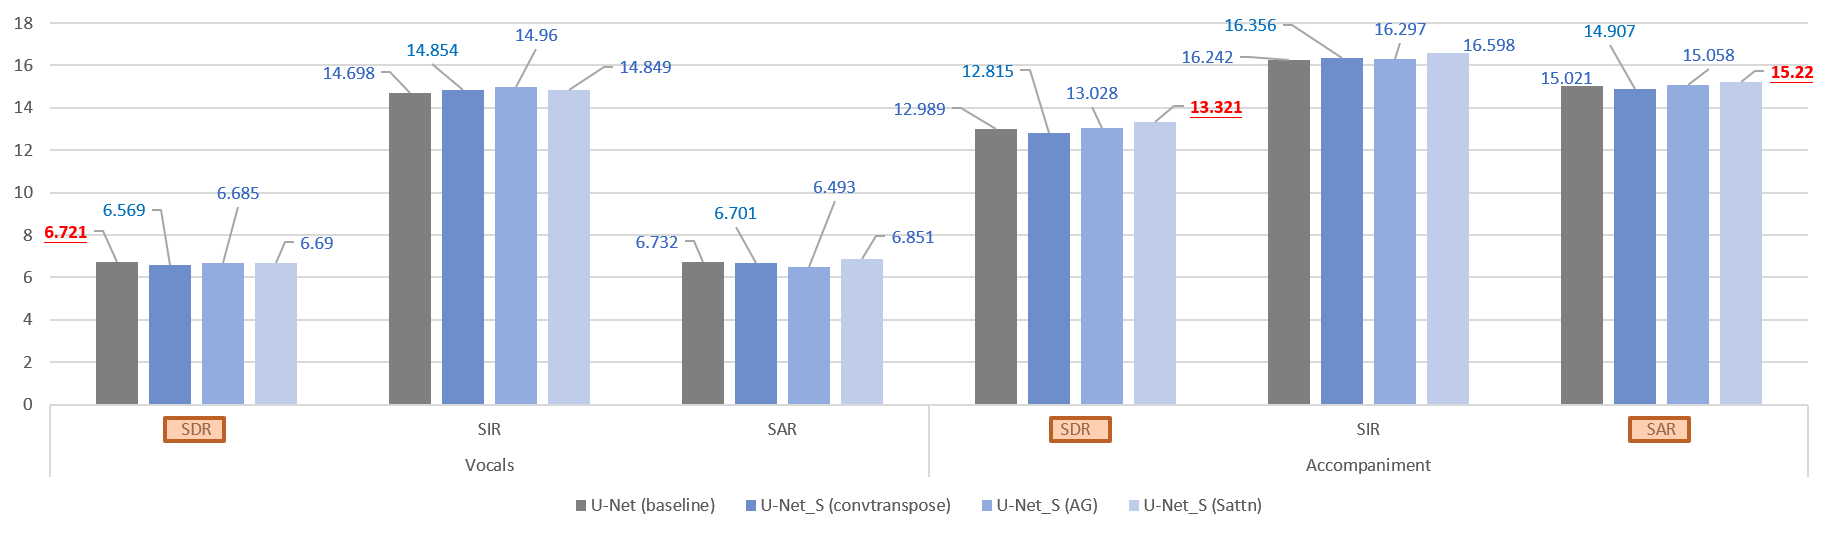
\includegraphics[width=\textwidth]{./figures/chapter05_result/attention_based_unet_result1.png}
        \caption {注意力模型的效果比較長條圖}
        \label{attention_based_unet_result1}
    \end{minipage}
    \hfil
\end{figure}

\begin{figure}[htbp]
    \hfil
    \begin{minipage}[t]{0.4\textwidth}
        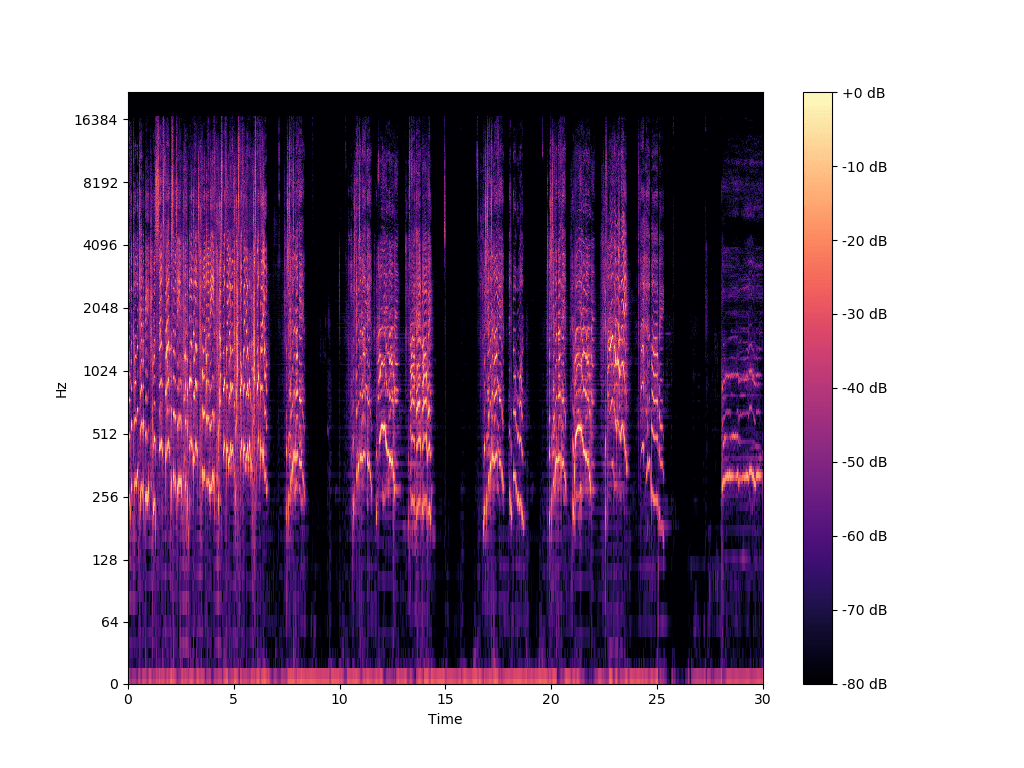
\includegraphics[width=\textwidth]{./figures/chapter05_result/6-Unet(base)_vocals.png}
        \caption {U-Net (baseline) 預測主唱音軌的頻譜圖}
        \label{U-Net6(baseline)_vocals}
    \end{minipage}
    \begin{minipage}[t]{0.4\textwidth}
        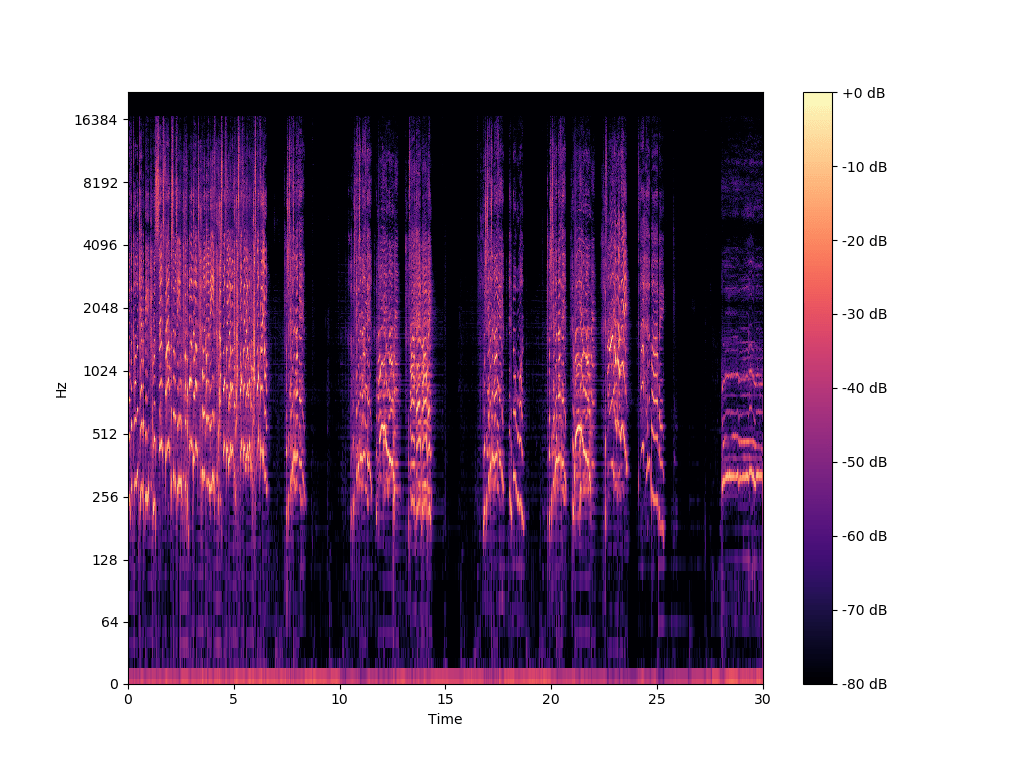
\includegraphics[width=\textwidth]{./figures/chapter05_result/6-Unet(Sattn_C-V4)_vocals.png}
        \caption {U-Net6 (Sattn) 預測主唱音軌的頻譜圖}
        \label{U-Net6(Sattn)_vocals}
    \end{minipage}
    \hfil
\end{figure}

\clearpage

\section{實驗四:模型剪枝效果比較}
模型剪枝的實驗中,表\ref{pruned_unet_table1} 記錄了 U-Net6(baseline)為基礎衍伸了兩個剪枝過後的模型,U-Net6\_s(DSConvB)與 U-Net6\_s(IRB),前者使用了深度可分卷積(Depthwise separable convolution),可以將模型大小縮為 18.71MB,後者使用 Inverted residual block 實現,可將模型大小縮為 59.8 MB。

\begin{table}[htbp]
\centering
\resizebox{\textwidth}{!}{%
\begin{tabular}{|r|c|c|l|}
\hline
 & Size (MB) & Normalization method & Note \\ \hline
U-Net6 (baseline) & 118.9 & Instance normalization &  \\ \hline
U-Net6\_s (DSConvB) & 18.71 & Batch normalization & DepthwiseSeparableConvBlock \\ \cline{1-2}
U-Net6\_s (IRB) & 59.8 &  & InvertedResidualBlock \\ \hline
\end{tabular}%
}
\caption{U-Net 的模型剪枝架構的比較}
\label{pruned_unet_table1}
\end{table}

\begin{table}[htbp]
\centering
\resizebox{\textwidth}{!}{%
\begin{tabular}{|r|l|l|l|l|}
\hline
 & Size (MB) & Up & Normalization method & Note \\ \hline
U-Net6\_s (baseline) & 118.9 & ConvT & Instance normalization & No scalability \\ \hline
U-Net6\_s (convtranspose) & 118.84 & ConvT & Instance normalization & Scalability, comparing set \\ \cline{1-4}
U-Net6\_s (upsample) & 88.08 & UpS & Instance normalization &  \\ \hline
U-Net6\_s (upsample-fusible) & 88.21 & UpS & Batch normalization & Scalability, quantization-ability \\ \hline
U-Net6\_s (DSConvB; convtranspose) & 18.71 & ConvT & Batch normalization & DepthwiseSeparableConvBlock \\ \cline{1-4}
U-Net6\_s (DSConvB; upsample) & 10.31 & UpS & Batch normalization &  \\ \hline
U-Net6\_s (IRB) & 59.8 & ConvT & Batch normalization & InvertedResidualishBlock \\ \hline
\end{tabular}%
}
\caption{模型剪枝過渡架構表}
\label{pruned_unet_table2}
\end{table}


\begin{figure}[htbp]
    \hfil
    \begin{minipage}[t]{0.45\textwidth}
        \centering
        % time series body
        \begin{tikzpicture}[scale=0.75]
        \begin{semilogyaxis} [
            xlabel = Epoch,
            ylabel = Loss,
        ]
            \addlegendentry{Training loss}
            \addplot table[mark=none, x=Step,y=Value, col sep=comma] {./numerical-data/chapter05_result/experiment04/6-Unet (base)/accompaniment/trnloss.csv};
            \addlegendentry{Validation loss}
            \addplot table[mark=none, x=Step,y=Value, col sep=comma] {./numerical-data/chapter05_result/experiment04/6-Unet (base)/accompaniment/valloss.csv};
        \end{semilogyaxis}
        \end{tikzpicture}
        % time series body
        \caption {U-Net6 (baseline) 對伴奏軌訓練的 loss}
        \label{e4:6-Unet (base):accompaniment}
    \end{minipage}
    \begin{minipage}[t]{0.45\textwidth}
        \centering
        % time series body
        \begin{tikzpicture}[scale=0.75]
        \begin{semilogyaxis} [
            xlabel = Epoch,
            ylabel = Loss,
        ]
            \addlegendentry{Training loss}
            \addplot table[mark=none, x=Step,y=Value, col sep=comma] {./numerical-data/chapter05_result/experiment04/6-Unet (base)/vocals/trnloss.csv};
            \addlegendentry{Validation loss}
            \addplot table[mark=none, x=Step,y=Value, col sep=comma] {./numerical-data/chapter05_result/experiment04/6-Unet (base)/vocals/valloss.csv};
        \end{semilogyaxis}
        \end{tikzpicture}
        % time series body
        \caption {U-Net6 (baseline) 對主唱軌訓練的 loss}
        \label{e4:6-Unet (base):vocals}
    \end{minipage}
    \hfil
\end{figure}

\begin{figure}[htbp]
    \hfil
    \begin{minipage}[t]{0.45\textwidth}
        \centering
        % time series body
        \begin{tikzpicture}[scale=0.75]
        \begin{semilogyaxis} [
            xlabel = Epoch,
            ylabel = Loss,
        ]
            \addlegendentry{Training loss}
            \addplot table[mark=none, x=Step,y=Value, col sep=comma] {./numerical-data/chapter05_result/experiment04/6-Unet (DSConvB)/accompaniment/trnloss.csv};
            \addlegendentry{Validation loss}
            \addplot table[mark=none, x=Step,y=Value, col sep=comma] {./numerical-data/chapter05_result/experiment04/6-Unet (DSConvB)/accompaniment/valloss.csv};
        \end{semilogyaxis}
        \end{tikzpicture}
        % time series body
        \caption {U-Net6\_s (DSConvB) 對伴奏軌訓練的 loss}
        \label{e4:6-Unet (DSConvB):accompaniment}
    \end{minipage}
    \begin{minipage}[t]{0.45\textwidth}
        \centering
        % time series body
        \begin{tikzpicture}[scale=0.75]
        \begin{semilogyaxis} [
            xlabel = Epoch,
            ylabel = Loss,
        ]
            \addlegendentry{Training loss}
            \addplot table[mark=none, x=Step,y=Value, col sep=comma] {./numerical-data/chapter05_result/experiment04/6-Unet (DSConvB)/vocals/trnloss.csv};
            \addlegendentry{Validation loss}
            \addplot table[mark=none, x=Step,y=Value, col sep=comma] {./numerical-data/chapter05_result/experiment04/6-Unet (DSConvB)/vocals/valloss.csv};
        \end{semilogyaxis}
        \end{tikzpicture}
        % time series body
        \caption {U-Net6\_s (DSConvB) 對主唱軌訓練的 loss}
        \label{e4:6-Unet (DSConvB):vocals}
    \end{minipage}
    \hfil
\end{figure}

\begin{figure}[htbp]
    \hfil
    \begin{minipage}[t]{0.45\textwidth}
        \centering
        % time series body
        \begin{tikzpicture}[scale=0.75]
        \begin{semilogyaxis} [
            xlabel = Epoch,
            ylabel = Loss,
        ]
            \addlegendentry{Training loss}
            \addplot table[mark=none, x=Step,y=Value, col sep=comma] {./numerical-data/chapter05_result/experiment04/6-Unet (IRB)/accompaniment/trnloss.csv};
            \addlegendentry{Validation loss}
            \addplot table[mark=none, x=Step,y=Value, col sep=comma] {./numerical-data/chapter05_result/experiment04/6-Unet (IRB)/accompaniment/valloss.csv};
        \end{semilogyaxis}
        \end{tikzpicture}
        % time series body
        \caption {U-Net6\_s (IRB) 對伴奏軌訓練的 loss}
        \label{e4:6-Unet (IRB):accompaniment}
    \end{minipage}
    \begin{minipage}[t]{0.45\textwidth}
        \centering
        % time series body
        \begin{tikzpicture}[scale=0.75]
        \begin{semilogyaxis} [
            xlabel = Epoch,
            ylabel = Loss,
        ]
            \addlegendentry{Training loss}
            \addplot table[mark=none, x=Step,y=Value, col sep=comma] {./numerical-data/chapter05_result/experiment04/6-Unet (IRB)/vocals/trnloss.csv};
            \addlegendentry{Validation loss}
            \addplot table[mark=none, x=Step,y=Value, col sep=comma] {./numerical-data/chapter05_result/experiment04/6-Unet (IRB)/vocals/valloss.csv};
        \end{semilogyaxis}
        \end{tikzpicture}
        % time series body
        \caption {U-Net6\_s (IRB) 對主唱軌訓練的 loss}
        \label{e4:6-Unet (IRB):vocals}
    \end{minipage}
    \hfil
\end{figure}


\begin{table}[htbp]
\centering
\resizebox{\textwidth}{!}{%
\begin{tabular}{|r|ccc|ccc|}
\hline
 &  & 主唱軌 &  &  & 伴奏軌 &  \\ \hline
 & \multicolumn{1}{c|}{\textbf{SDR}} & \multicolumn{1}{c|}{SIR} & SAR & \multicolumn{1}{c|}{\textbf{SDR}} & \multicolumn{1}{c|}{SIR} & \textbf{SAR} \\ \hline
\textit{U-Net6 (baseline)} & \multicolumn{1}{c|}{\textit{6.721}} & \multicolumn{1}{c|}{\textit{14.698}} & \textit{6.732} & \multicolumn{1}{c|}{\textit{12.989}} & \multicolumn{1}{c|}{\textit{16.242}} & \textit{15.021} \\ \hline
U-Net6\_s (DSConvB; convtranspose) & \multicolumn{1}{c|}{5.981} & \multicolumn{1}{c|}{14.169} & 6.044 & \multicolumn{1}{c|}{12.308} & \multicolumn{1}{c|}{16.016} & 14.143 \\ \hline
U-Net\_s (IRB) & \multicolumn{1}{c|}{\textbf{6.51}} & \multicolumn{1}{c|}{13.989} & 6.486 & \multicolumn{1}{c|}{\textbf{12.771}} & \multicolumn{1}{c|}{15.985} & \textbf{14.769} \\ \hline
\end{tabular}%
}
\caption{模型剪枝的效果比較表}
\label{pruned_unet_table3}
\end{table}

\begin{figure}[htbp]
    \hfil
    \begin{minipage}[t]{1.0\textwidth}
        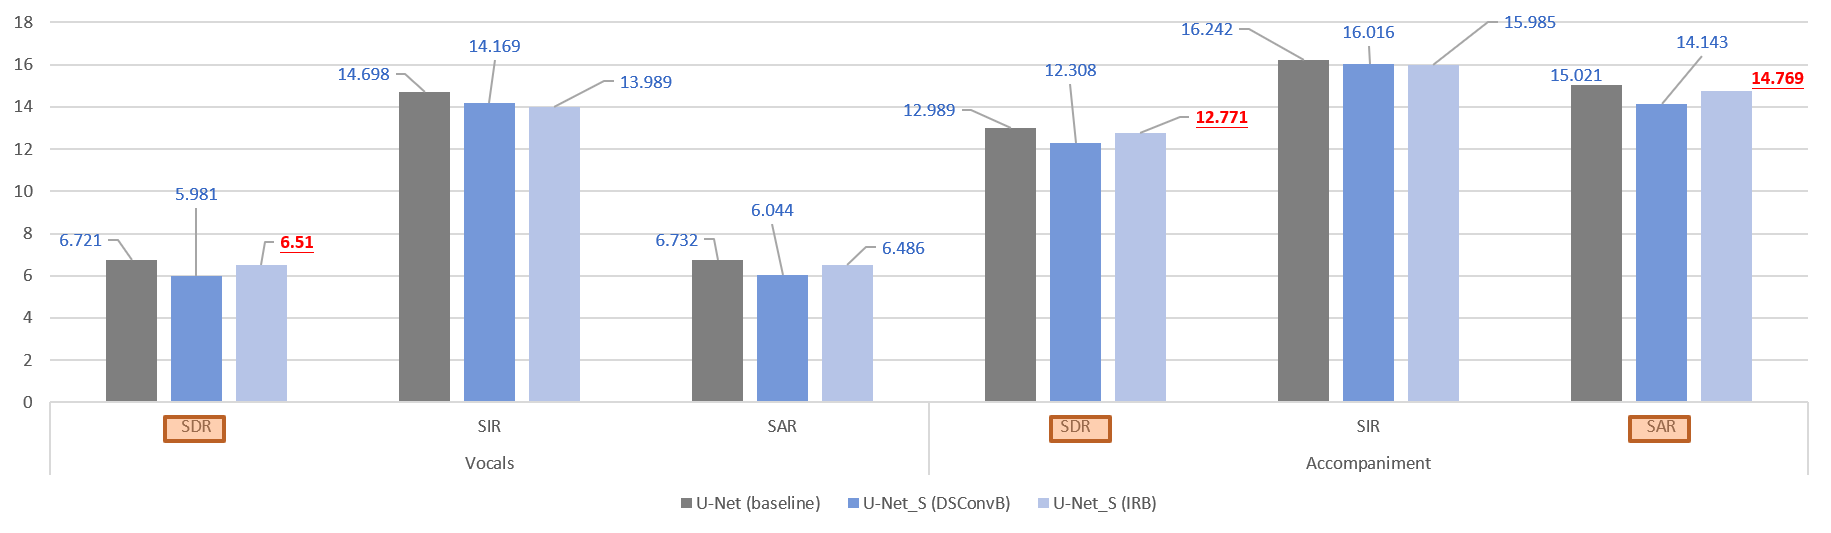
\includegraphics[width=\textwidth]{./figures/chapter05_result/pruned_unet_result1.png}
        \caption {模型剪枝的效果比較長條圖}
        \label{pruned_unet_result1}
    \end{minipage}
    \hfil
\end{figure}

\clearpage

\section{實驗五:模型量化效果比較}
% 量化結果有時間的話應仍要在完整的 Musdb18 中測試其 metrics
量化實驗中,要從所有的候選模型中挑選(表\ref{quantization_table1} 與表 \ref{quantization_table2} ),本實驗選擇三個模型做量化,分別是:U-Net6\_s(upsample)、U-Net6\_s(DSConvB; convtranspose)與 U-Net6\_s (IRB),並使用 QNNPACK~\cite{dukhan2018qnnpack,wu2019machine} 實現。U-Net6\_s(upsample) 是模型量化實驗中,用來  評估基準模型量化過後的能力,為 U-Net6(baseline) 的微調版本。選擇 U-Net6\_s(DSConvB; convtranspose)的原因是模型參數最少,而使用 convtranspose 的狀態又比使用 upsample 時還要好,固選之。選擇 U-Net6 (IRB) 是因為其模型參數量介於中間,用來作為比較使用。

以下模型:U-Net6\_s(upsample)(表\ref{quantization_table3}與圖\ref{quantization_result1})、U-Net6\_s(DSConvB; convtranspose)(表\ref{quantization_table4}與圖\ref{quantization_result2})與 U-Net6 (IRB)(表\ref{quantization_table5}與圖\ref{quantization_result3})。以訓練的模型再使用 Musdb18 的七秒資料集中做「校準」,最後使用該資料及與 museval 測試量化後的效果。Musdb18 的七秒資料集是官方將原本資料集的每首歌做裁減,縮小該資料集,在本實驗中的校準階段需要大量的時間,以該資料集可不失歌曲種類的多樣性,但也可很好得量化模型。

\begin{table}[htbp]
\centering
\resizebox{\textwidth}{!}{%
\begin{tabular}{|r|c|c|c|l|}
\hline
 & Size (MB) & Up & Normalization method & Note \\ \hline
U-Net6 (baseline) & 118.9 & ConvT & Instance normalization & No scalability \\ \hline
U-Net6\_s (convtranspose) & 118.84 & ConvT & Instance normalization & Scalability, comparing set \\ \cline{1-4}
U-Net6\_s (upsample) & 88.08 & UpS & Instance normalization &  \\ \hline
U-Net6\_s (upsample-fusible) & 88.21 & UpS & Batch normalization & Scalability, quantization-ability \\ \hline
\textbf{U-Net6\_s (DSConvB; convtranspose)} & \textbf{18.71} & ConvT & Batch normalization & DepthwiseSeparableConvBlock \\ \cline{1-4}
U-Net6\_s (DSConv; upsample) & 10.31 & UpS & Batch normalization &  \\ \hline
\textbf{U-Net6\_s (IRB)} & \textbf{59.8} & ConvT & Batch normalization & InvertedResidualishBlock \\ \hline
\end{tabular}%
}
\caption{模型量化的候選表}
\label{quantization_table1}
\end{table}

\begin{table}[htbp]
\centering
\resizebox{\textwidth}{!}{%
\begin{tabular}{|r|ccc|ccc|}
\hline
 &  & 主唱軌 &  &  & 伴奏軌 &  \\ \hline
 & \multicolumn{1}{c|}{\textbf{SDR}} & \multicolumn{1}{c|}{SIR} & SAR & \multicolumn{1}{c|}{\textbf{SDR}} & \multicolumn{1}{c|}{SIR} & \textbf{SAR} \\ \hline
\textit{U-Net6 (baseline)} & \multicolumn{1}{c|}{\textit{6.721}} & \multicolumn{1}{c|}{\textit{14.698}} & \textit{6.732} & \multicolumn{1}{c|}{\textit{12.989}} & \multicolumn{1}{c|}{\textit{16.242}} & \textit{15.021} \\ \hline
U-Net6\_s (convtranspose) & \multicolumn{1}{c|}{6.569} & \multicolumn{1}{c|}{14.854} & 6.701 & \multicolumn{1}{c|}{12.815} & \multicolumn{1}{c|}{16.356} & 14.907 \\ \hline
U-Net6\_s (upsample) & \multicolumn{1}{c|}{6.553} & \multicolumn{1}{c|}{13.986} & 6.383 & \multicolumn{1}{c|}{13.013} & \multicolumn{1}{c|}{16.412} & 14.746 \\ \hline
U-Net6\_s (upsample-fusible) & \multicolumn{1}{c|}{6.612} & \multicolumn{1}{c|}{14.66} & 6.845 & \multicolumn{1}{c|}{12.918} & \multicolumn{1}{c|}{16.226} & 14.932 \\ \hline
\textbf{U-Net6 (DSConvB; convtranspose)} & \multicolumn{1}{c|}{5.981} & \multicolumn{1}{c|}{14.169} & 6.044 & \multicolumn{1}{c|}{12.308} & \multicolumn{1}{c|}{16.016} & 14.143 \\ \hline
U-Net6 (DSConvB; upsample) & \multicolumn{1}{c|}{5.922} & \multicolumn{1}{c|}{13.925} & 5.929 & \multicolumn{1}{c|}{12.278} & \multicolumn{1}{c|}{15.653} & 14.325 \\ \hline
\textbf{U-Net6 (IRB)} & \multicolumn{1}{c|}{6.51} & \multicolumn{1}{c|}{13.989} & 6.486 & \multicolumn{1}{c|}{12.771} & \multicolumn{1}{c|}{15.985} & 14.769 \\ \hline
\end{tabular}%
}
\caption{模型量化候選模型的效果表}
\label{quantization_table2}
\end{table}

\begin{table}[htbp]
\centering
\resizebox{\textwidth}{!}{%
\begin{tabular}{|r|ccc|ccc|}
\hline
 &  & 主唱軌 &  &  & 伴奏軌 &  \\ \hline
 & \multicolumn{1}{c|}{\textbf{SDR}} & \multicolumn{1}{c|}{SIR} & SAR & \multicolumn{1}{c|}{\textbf{SDR}} & \multicolumn{1}{c|}{SIR} & \textbf{SAR} \\ \hline
\textit{U-Net6\_s (upsample-fusible)} & \multicolumn{1}{c|}{\textit{7.275}} & \multicolumn{1}{c|}{\textit{11.228}} & \textit{8.259} & \multicolumn{1}{c|}{\textit{12.17}} & \multicolumn{1}{c|}{\textit{14.795}} & \textit{15.057} \\ \hline
Default quantization & \multicolumn{1}{c|}{6.919} & \multicolumn{1}{c|}{11.374} & 8.115 & \multicolumn{1}{c|}{\textbf{11.813}} & \multicolumn{1}{c|}{14.254} & 14.569 \\ \hline
Advance quantization & \multicolumn{1}{c|}{\textbf{7.160}} & \multicolumn{1}{c|}{11.082} & 8.096 & \multicolumn{1}{c|}{11.551} & \multicolumn{1}{c|}{13.848} & \textbf{14.866} \\ \hline
\end{tabular}%
}
\caption{U-Net6\_s(upsample-fusible)量化效果表}
Model size: 88.21 (MB) vs. 22.09 (MB)
\label{quantization_table3}
\end{table}


\begin{figure}[htbp]
    \hfil
    \begin{minipage}[t]{1.0\textwidth}
        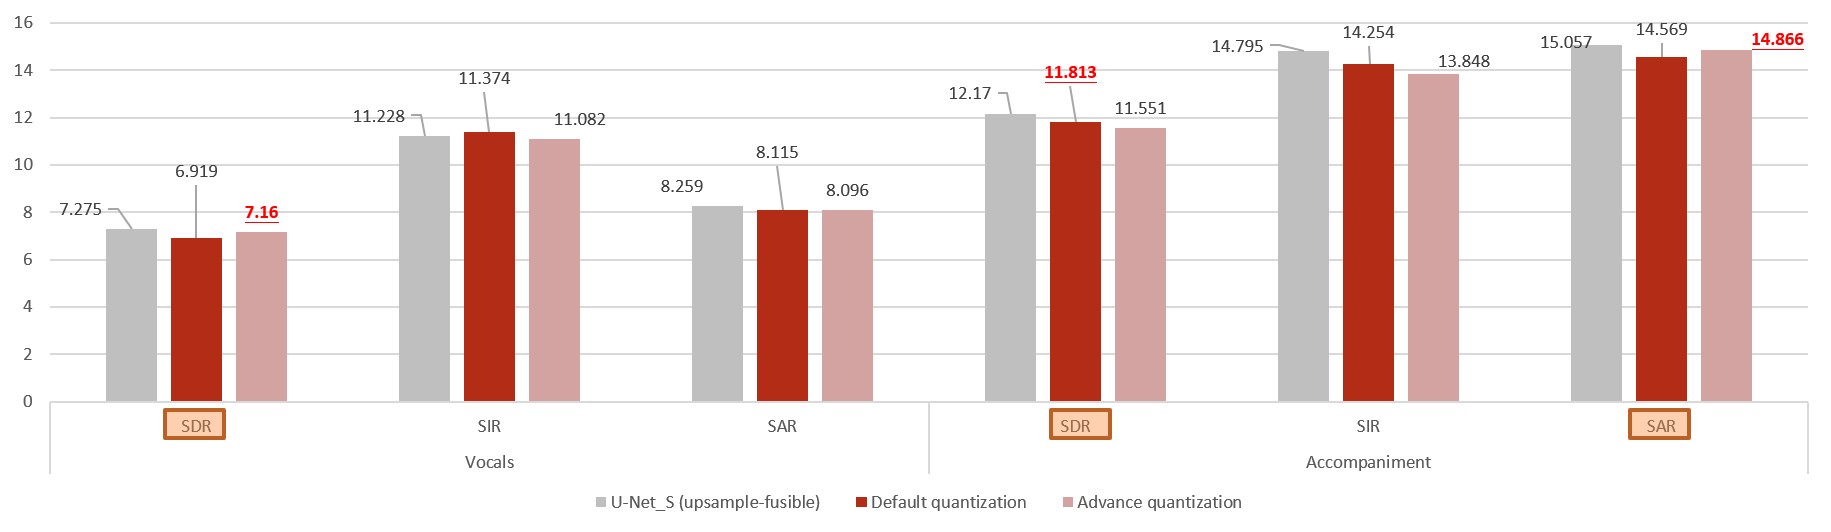
\includegraphics[width=\textwidth]{./figures/chapter05_result/quantization_result1.png}
        \caption {U-Net6\_s(upsample-fusible)量化效果長條圖}
        \label{quantization_result1}
    \end{minipage}
    \hfil
\end{figure}


\begin{table}[htbp]
\centering
\resizebox{\textwidth}{!}{%
\begin{tabular}{|r|ccc|ccc|}
\hline
 &  & 主唱軌 &  &  & 伴奏軌 &  \\ \hline
 & \multicolumn{1}{c|}{\textbf{SDR}} & \multicolumn{1}{c|}{SIR} & SAR & \multicolumn{1}{c|}{\textbf{SDR}} & \multicolumn{1}{c|}{SIR} & \textbf{SAR} \\ \hline
\textit{U-Net6\_s (DSConvB; convtranspose)} & \multicolumn{1}{c|}{\textit{6.648}} & \multicolumn{1}{c|}{\textit{11.019}} & \textit{7.471} & \multicolumn{1}{c|}{\textit{11.428}} & \multicolumn{1}{c|}{\textit{14.54}} & \textit{14.171} \\ \hline
Default quantization & \multicolumn{1}{c|}{3.028} & \multicolumn{1}{c|}{11.214} & 7.143 & \multicolumn{1}{c|}{\textbf{11.184}} & \multicolumn{1}{c|}{14.92} & \textbf{13.993} \\ \hline
Advance quantization & \multicolumn{1}{c|}{\textbf{5.87}} & \multicolumn{1}{c|}{10.424} & 7.306 & \multicolumn{1}{c|}{11.041} & \multicolumn{1}{c|}{14.357} & 13.655 \\ \hline
\end{tabular}%
}
\caption{U-Net6\_s(DSConvB; convtranspose)量化效果表}
Model size: 18.71 (MB) vs. 4.75 (MB)
\label{quantization_table4}
\end{table}

\begin{figure}[htbp]
    \hfil
    \begin{minipage}[t]{1.0\textwidth}
        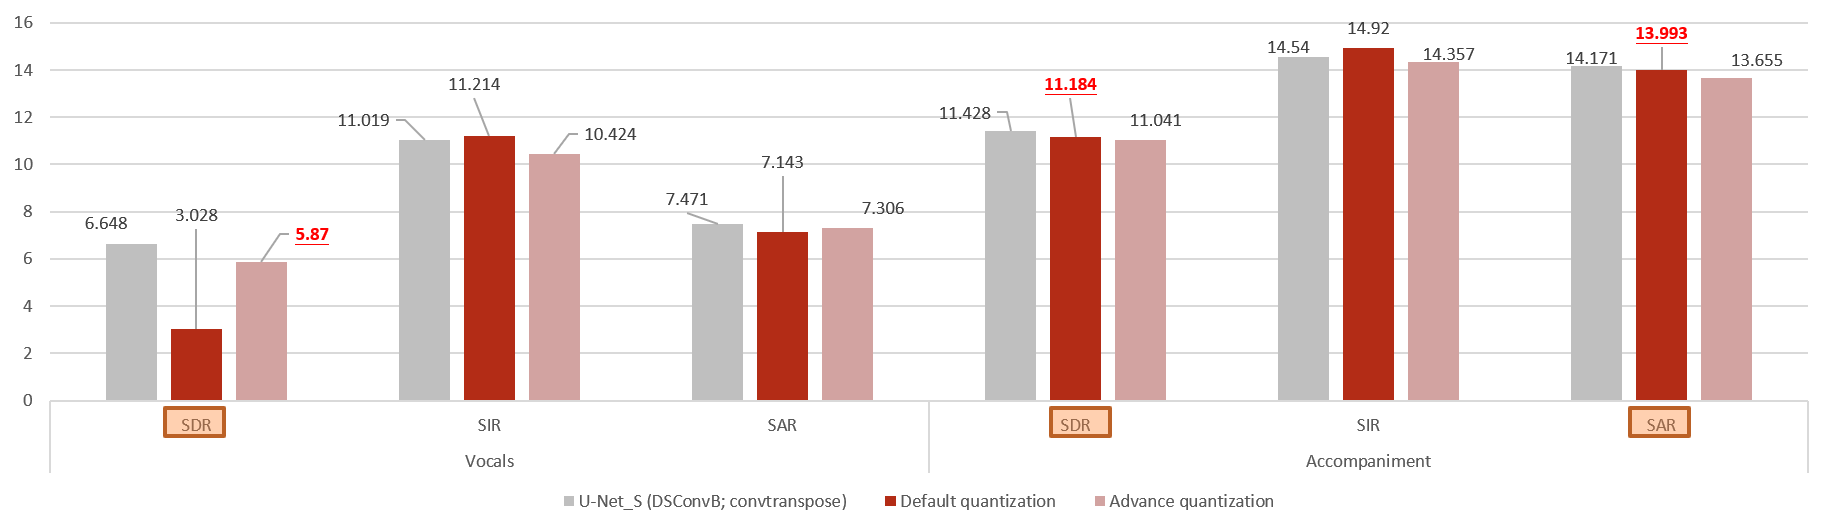
\includegraphics[width=\textwidth]{./figures/chapter05_result/quantization_result2.png}
        \caption {U-Net6\_s(DSConvB; convtranspose)量化效果長條圖}
        \label{quantization_result2}
    \end{minipage}
    \hfil
\end{figure}

\begin{table}[htbp]
\centering
\resizebox{\textwidth}{!}{%
\begin{tabular}{|r|ccc|ccc|}
\hline
 &  & 主唱軌 &  &  & 伴奏軌 &  \\ \hline
 & \multicolumn{1}{c|}{\textbf{SDR}} & \multicolumn{1}{c|}{SIR} & SAR & \multicolumn{1}{c|}{\textbf{SDR}} & \multicolumn{1}{c|}{SIR} & \textbf{SAR} \\ \hline
\textit{U-Net6\_s (IRB)} & \multicolumn{1}{c|}{\textit{6.691}} & \multicolumn{1}{c|}{\textit{10.75}} & \textit{8.166} & \multicolumn{1}{c|}{\textit{11.816}} & \multicolumn{1}{c|}{\textit{14.829}} & \textit{15.021} \\ \hline
Default quantization & \multicolumn{1}{c|}{\textbf{6.446}} & \multicolumn{1}{c|}{10.345} & 7.895 & \multicolumn{1}{c|}{6.009} & \multicolumn{1}{c|}{14.799} & 8.969 \\ \hline
Advance quantization & \multicolumn{1}{c|}{6.362} & \multicolumn{1}{c|}{10.361} & 7.728 & \multicolumn{1}{c|}{\textbf{11.048}} & \multicolumn{1}{c|}{15.059} & \textbf{13.6} \\ \hline
\end{tabular}%
}
\caption{U-Net6\_s (IRB) 量化效果表}
Model size: 59.80 (MB) vs. 15.07 (MB)
\label{quantization_table5}
\end{table}

\begin{figure}[htbp]
    \hfil
    \begin{minipage}[t]{1.0\textwidth}
        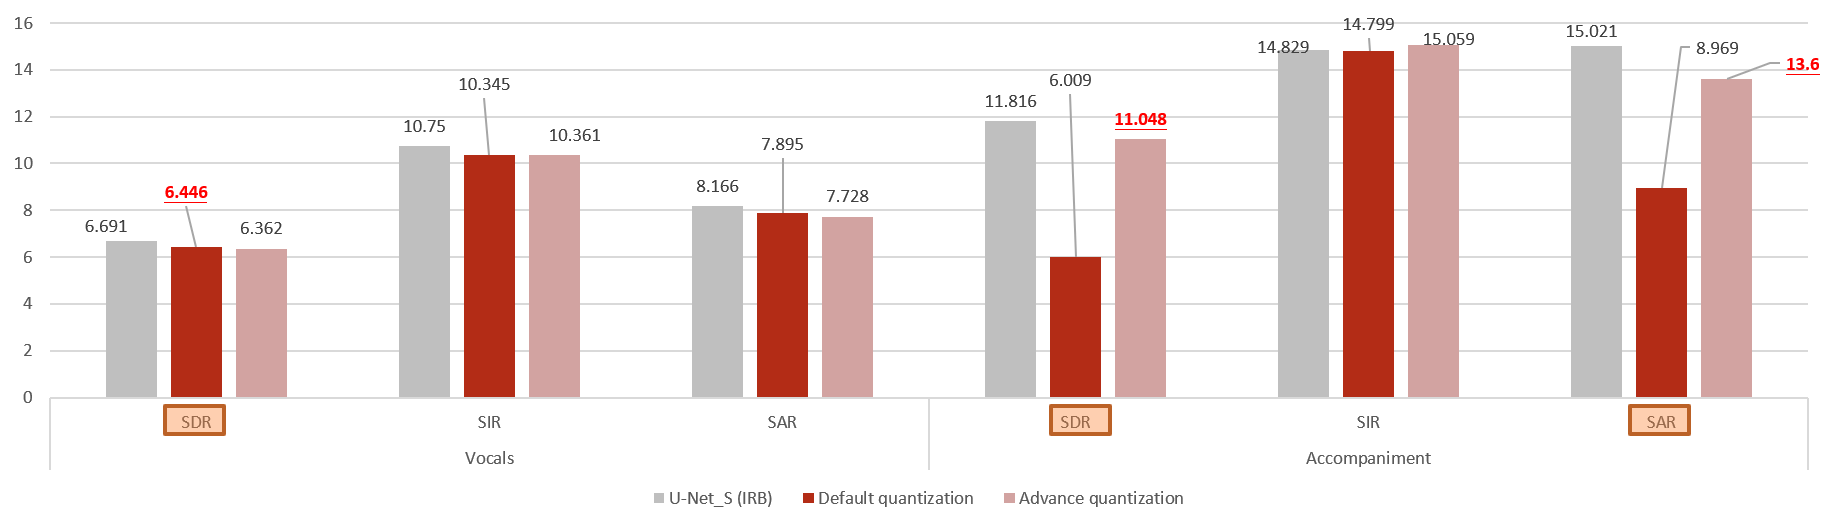
\includegraphics[width=\textwidth]{./figures/chapter05_result/quantization_result3.png}
        \caption {U-Net6\_s (IRB) 量化效果長條圖}
        \label{quantization_result3}
    \end{minipage}
    \hfil
\end{figure}